%%%%%%%%%%%%%%%%%%%%%%%%%%%%%%%%%%%%%%%%%
% Beamer Presentation
% LaTeX Template
% Version 1.0 (10/11/12)
%
% This template has been downloaded from:
% http://www.LaTeXTemplates.com
%
% License:
% CC BY-NC-SA 3.0 (http://creativecommons.org/licenses/by-nc-sa/3.0/)
%
%%%%%%%%%%%%%%%%%%%%%%%%%%%%%%%%%%%%%%%%%

%----------------------------------------------------------------------------------------
%	PACKAGES AND THEMES
%----------------------------------------------------------------------------------------

\documentclass{beamer}

\mode<presentation> {

% The Beamer class comes with a number of default slide themes
% which change the colors and layouts of slides. Below this is a list
% of all the themes, uncomment each in turn to see what they look like.

%\usetheme{default}
%\usetheme{AnnArbor}
%\usetheme{Antibes}
%\usetheme{Bergen}
%\usetheme{Berkeley}
%\usetheme{Berlin}
%\usetheme{Boadilla}
%\usetheme{CambridgeUS}
%\usetheme{Copenhagen}
%\usetheme{Darmstadt}
%\usetheme{Dresden}
%\usetheme{Frankfurt}
%\usetheme{Goettingen}
%\usetheme{Hannover}
%\usetheme{Ilmenau}
%\usetheme{JuanLesPins}
%\usetheme{Luebeck}
\usetheme{Madrid} %i was using this one
%\usetheme{Malmoe}
%\usetheme{Marburg}
%\usetheme{Montpellier}
%\usetheme{PaloAlto}
%\usetheme{Pittsburgh}
%\usetheme{Rochester}
%\usetheme{Singapore}
%\usetheme{Szeged}
%\usetheme{Warsaw}

% As well as themes, the Beamer class has a number of color themes
% for any slide theme. Uncomment each of these in turn to see how it
% changes the colors of your current slide theme.

%\usecolortheme{albatross}
%\usecolortheme{beaver}
%\usecolortheme{beetle}
%\usecolortheme{crane}
%\usecolortheme{dolphin}
%\usecolortheme{dove}
%\usecolortheme{fly}
%\usecolortheme{lily}
%\usecolortheme{orchid}
%\usecolortheme{rose}
%\usecolortheme{seagull}
%\usecolortheme{seahorse}
%\usecolortheme{whale}
%\usecolortheme{wolverine}

%\setbeamertemplate{footline} % To remove the footer line in all slides uncomment this line
%\setbeamertemplate{footline}[page number] % To replace the footer line in all slides with a simple slide count uncomment this line

%\setbeamertemplate{navigation symbols}{} % To remove the navigation symbols from the bottom of all slides uncomment this line
}

\usepackage{graphicx} % Allows including images
\usepackage{booktabs} % Allows the use of \toprule, \midrule and \bottomrule in tables
\usepackage{hyperref}

%----------------------------------------------------------------------------------------
%	TITLE PAGE
%----------------------------------------------------------------------------------------

\title[Course Intro]{Introduction to Methods in Computational Biology and Genomics} % The short title appears at the bottom of every slide, the full title is only on the title page

\author{C. Ryan Campbell} % Your name
\institute[Duke] % Your institution as it will appear on the bottom of every slide, may be shorthand to save space
{
Duke University \\ % Your institution for the title page
\medskip
\textit{c.ryan.campbell@duke.edu} % Your email address
}
\date{\today} % Date, can be changed to a custom date

\begin{document}

\begin{frame}
\titlepage % Print the title page as the first slide
\end{frame}

\begin{frame}
\frametitle{Overview} % Table of contents slide, comment this block out to remove it
\tableofcontents % Throughout your presentation, if you choose to use \section{} and \subsection{} commands, these will automatically be printed on this slide as an overview of your presentation
\end{frame}

%----------------------------------------------------------------------------------------
%	PRESENTATION SLIDES
%----------------------------------------------------------------------------------------

%------------------------------------------------
\section{Course} % Sections can be created in order to organize your presentation into discrete blocks, all sections and subsections are automatically printed in the table of contents as an overview of the talk
%------------------------------------------------

\subsection{Course Intro} % A subsection can be created just before a set of slides with a common theme to further break down your presentation into chunks

%------------------------------------------------
\begin{frame}
\frametitle{Today's Goals}
%what students should know/learn today
\begin{itemize}
\item Get familiarized with course format
\item Meet each other and myself
\item Understand course expectations
%\ttfamily
\item Know my teaching methods and reasons for offering this course
%\sffamily
\end{itemize}


\end{frame}
%------------------------------------------------
\begin{frame}
\frametitle{Course Objectives}
%modified from syllabus
\begin{block}{Objective 1}<1->
Learning programming basics and best practices within a biology framework (i.e. basic building blocks for students to use biological software)
\end{block}

\begin{block}{Objective 2}<2->
Learning the statistics that underlie these tools and the rapidly evolving suite of measures used in "genomics"
\end{block}

\begin{block}{Objective 3}<3->
Combine 1 and 2 to test biological hypotheses with RNAseq data and present those results in an "IMRD" format (pronounced EM-rod)
\end{block}


\end{frame}
%------------------------------------------------
\begin{frame}
\frametitle{Course Syllabus}
%go over main points
%from syllabus
\end{frame}
%------------------------------------------------
\begin{frame}
\frametitle{Course Grade}
%largely project based, partial throughout semester
%randomly based on class activity
%pick allotment
\end{frame}
%------------------------------------------------
\begin{frame}
\frametitle{Course Policies}
\begin{itemize}
\item<1-> Group Work vs. Own Work
\item<2-> No Direct Attendence Policy
\item<3-> Interact and Contribute in Class
\end{itemize}

%group work v. own work

%no direct attendence policy (but i reserve the right to add one)
\end{frame}
%------------------------------------------------
\begin{frame}
\frametitle{Potential Course Policies - TBD}
\begin{itemize}
\item<1-> Latest pre-class email time (5pm? 9pm?)
\item<2-> Slack?
\end{itemize}
%
\end{frame}
%------------------------------------------------

\begin{frame}
\frametitle{Day-to-day Course}
\begin{itemize}
\item<1-> Bring a laptop
\begin{itemize}
	\item<2-> Yes, Every Day
\end{itemize}
\item<3-> Tuesdays = Lecture
\item<4-> Thursdays = Lab
\end{itemize}
%bring a laptop
%Tues/Thurs
\end{frame}
%------------------------------------------------
\begin{frame}
\frametitle{Project}
\end{frame}
%------------------------------------------------

\subsection{Teaching Philosophy}
%------------------------------------------------
\begin{frame}
\frametitle{Teaching Philosophy}
\begin{itemize}
	\item Clear Goals
	\item Active Learning
	\item Student Driven
\end{itemize}

\end{frame}
%------------------------------------------------
\begin{frame}
\frametitle{Clear Goals}
\begin{itemize}
	\item Presented before each class
	\item Concepts or skills to focus on
	\item Call me on it if I forget them
\end{itemize}
%
\end{frame}
%------------------------------------------------
\begin{frame}
\frametitle{Active Learning}
\begin{itemize}
	\item Student Participation
	\item A different style than lecture-based courses (flipped courses fall into this category)
	\item Natural fit for smaller class size, advanced material, and learning skills
\end{itemize}

%
\end{frame}
%------------------------------------------------
\begin{frame}
\frametitle{Student Driven}
\begin{itemize}
	\item Student Participation Required
	\item Work through examples in class and apply to your own question
	\item Many skills need to be practiced, not taught
	\item Grand Bargain
	%bargain - i will try to avoid boring step by step tutorials where you just copy and paste
	% but you have to actually do the activities and learn actively
\end{itemize}

\end{frame}
%------------------------------------------------



\section{In-Class Activity}
%------------------------------------------------

\begin{frame}
\frametitle{In-Class Activity}
	\begin{enumerate}
	\item<1-> Pair up *randomly*
	\item<2-> Fill out this \href{https://goo.gl/forms/fnCaNIcwQiNiawcv1}{Google form}
	\item<3-> Make a slide in the \href{https://docs.google.com/presentation/d/1WxVQJGrBO8NxQ2ZJwvZy2W61qAQYqN9V8a_xRUflU7w/edit?usp=sharing}{Google Slideshow} for your partner with their answers, including (at minimum):
		\begin{itemize}
		\item<4-> Name
		\item<4-> Picture
		\item<4-> `Three words' response
		\item<4-> Two answers from `'Whimsy'
		\item<4-> Feel free to expand (see \href{https://docs.google.com/presentation/d/1WxVQJGrBO8NxQ2ZJwvZy2W61qAQYqN9V8a_xRUflU7w/edit?usp=sharing}{my slide} for reference)
		\end{itemize}
	\item<5-> Introduce partner to class
	\end{enumerate}
\end{frame}

%------------------------------------------------
\section{Computing and Genomics}
\subsection{Computer Requirements}
%------------------------------------------------
\begin{frame}
\frametitle{Computer Requirements}
\begin{itemize}
	\item Bring your computer to class
	\item Run some software locally
	\begin{itemize}
		\item How much storage do your computers have?
	\end{itemize}
	\item Connect to cluster
\end{itemize}
%bring yours to every class
%run software from your computer
\end{frame}
%------------------------------------------------
\begin{frame}
\frametitle{Research Tools}
\begin{itemize}
	\item<1-> R
	\begin{itemize}
	\item<1-> Statistical software, data visualization and analysis
	\end{itemize}
	\item<2-> kallisto
	\begin{itemize}
	\item<2-> Fast RNAseq analysis with a command line interface
	\end{itemize}	
	\item<3-> github
	\begin{itemize}
	\item<3-> Website for version control as well as script and code storage
	\end{itemize}
\end{itemize}
\end{frame}
%------------------------------------------------
\begin{frame}
\frametitle{Programming Languages}
\begin{itemize}
	\item R
	\begin{itemize}
		\item free statistical software
	\end{itemize}
	\item bin/bash
	\begin{itemize}
		\item unix language, automate many tasks, interact with cluster computers
	\end{itemize}
\end{itemize}
\end{frame}
%------------------------------------------------
\begin{frame}
\frametitle{Software}
\begin{itemize}
	\item<1-> R -> R-Studio
	\item<2-> github -> SourceTree
	\item<3-> data analysis software -> fastqc/trimmomatic/kallisto
\end{itemize}
\end{frame}
%------------------------------------------------
\begin{frame}
\frametitle{Cluster Computing}
\begin{itemize}
	\item Duke Computing Cluster
	\item SLURM workload manager
\end{itemize}
\end{frame}
%------------------------------------------------

\subsection{Genomics: Why We're Here}
%------------------------------------------------
\begin{frame}
\frametitle{Hand Raising Request}
\begin{itemize}
	\item<1-> Student Driven - Active Learning
	\item<2-> Raise your hand if you're confused
	\item<3-> Provides me with helpful feedback
\end{itemize}
%Student Driven
%
\end{frame}
%------------------------------------------------
\begin{frame}
\frametitle{What is/are Genomics?}
\begin{itemize}
	\item<2-> Within the field of molecular biology, genomics is the study of genomes, the complete set of genetic material within an organism.
	\item<3-> Genomics involves the sequencing and analysis of genomes. 
	\item<4-> Genomics is also concerned with the structure, function, comparison, and evolution of genomes.
	\item<5-> The field also includes studies of intragenomic (within the genome) phenomena such as heterosis (hybrid vigour), epistasis (effect of one gene on another), pleiotropy (one gene affecting more than one trait) and other interactions between loci and alleles within the genome.
	\item<6-> In contrast to genetics, which refers to the study of individual genes and their roles in inheritance, genomics uses high throughput DNA sequencing and bioinformatics to assemble, and analyze the function and structure of entire genomes.
\end{itemize}
\end{frame}
%------------------------------------------------
\begin{frame}
\frametitle{Brief History of Sequencing}
\begin{itemize}
	\item Allozymes
	\begin{itemize}
		\item Electrophoresis separates different proteins by amino acid makeup
	\end{itemize}
	\item Sanger Sequencing
	\begin{itemize}
		\item Determines the sequences a single piece of DNA up to 500bp
	\end{itemize}
	\item NGS - Next Generation Sequencing
	\begin{itemize}
		\item Reads sequence of many pieces of DNA many billions of times
	\end{itemize}
\end{itemize}
\end{frame}
%------------------------------------------------
\begin{frame}
\frametitle{Brief History of Sequencing}
\begin{itemize}
	\item Allozymes
	\begin{itemize}
		\item 1960's
	\end{itemize}
	\item Sanger Sequencing
	\begin{itemize}
		\item 1977
	\end{itemize}
	\item NGS - Next Generation Sequencing
	\begin{itemize}
		\item 2000
	\end{itemize}
\end{itemize}
\end{frame}
%------------------------------------------------

\begin{frame}
\frametitle{Next Generation Sequencing vs. Sanger}
\begin{itemize}
	\item<1-> Output for Quality Tradeoff
	\begin{itemize}
		\item NGS = High Output / Lower Quality
		\item Sanger = Low Output / High Quality
	\end{itemize}
	\item<2-> NGS Methods and Machines
	\begin{itemize}
		\item<3-> PyroSeq
		\item IonTorrent
		\item Illumina
		\item PacBio
	\end{itemize}
\end{itemize}
\end{frame}
%------------------------------------------------
\begin{frame}
\begin{figure}

\includegraphics[width=0.8\linewidth]{images_20170829_NGS_meme.png}
\end{figure}
\end{frame}
%------------------------------------------------
\begin{frame}
\frametitle{Sequencing Cost}
\begin{figure}
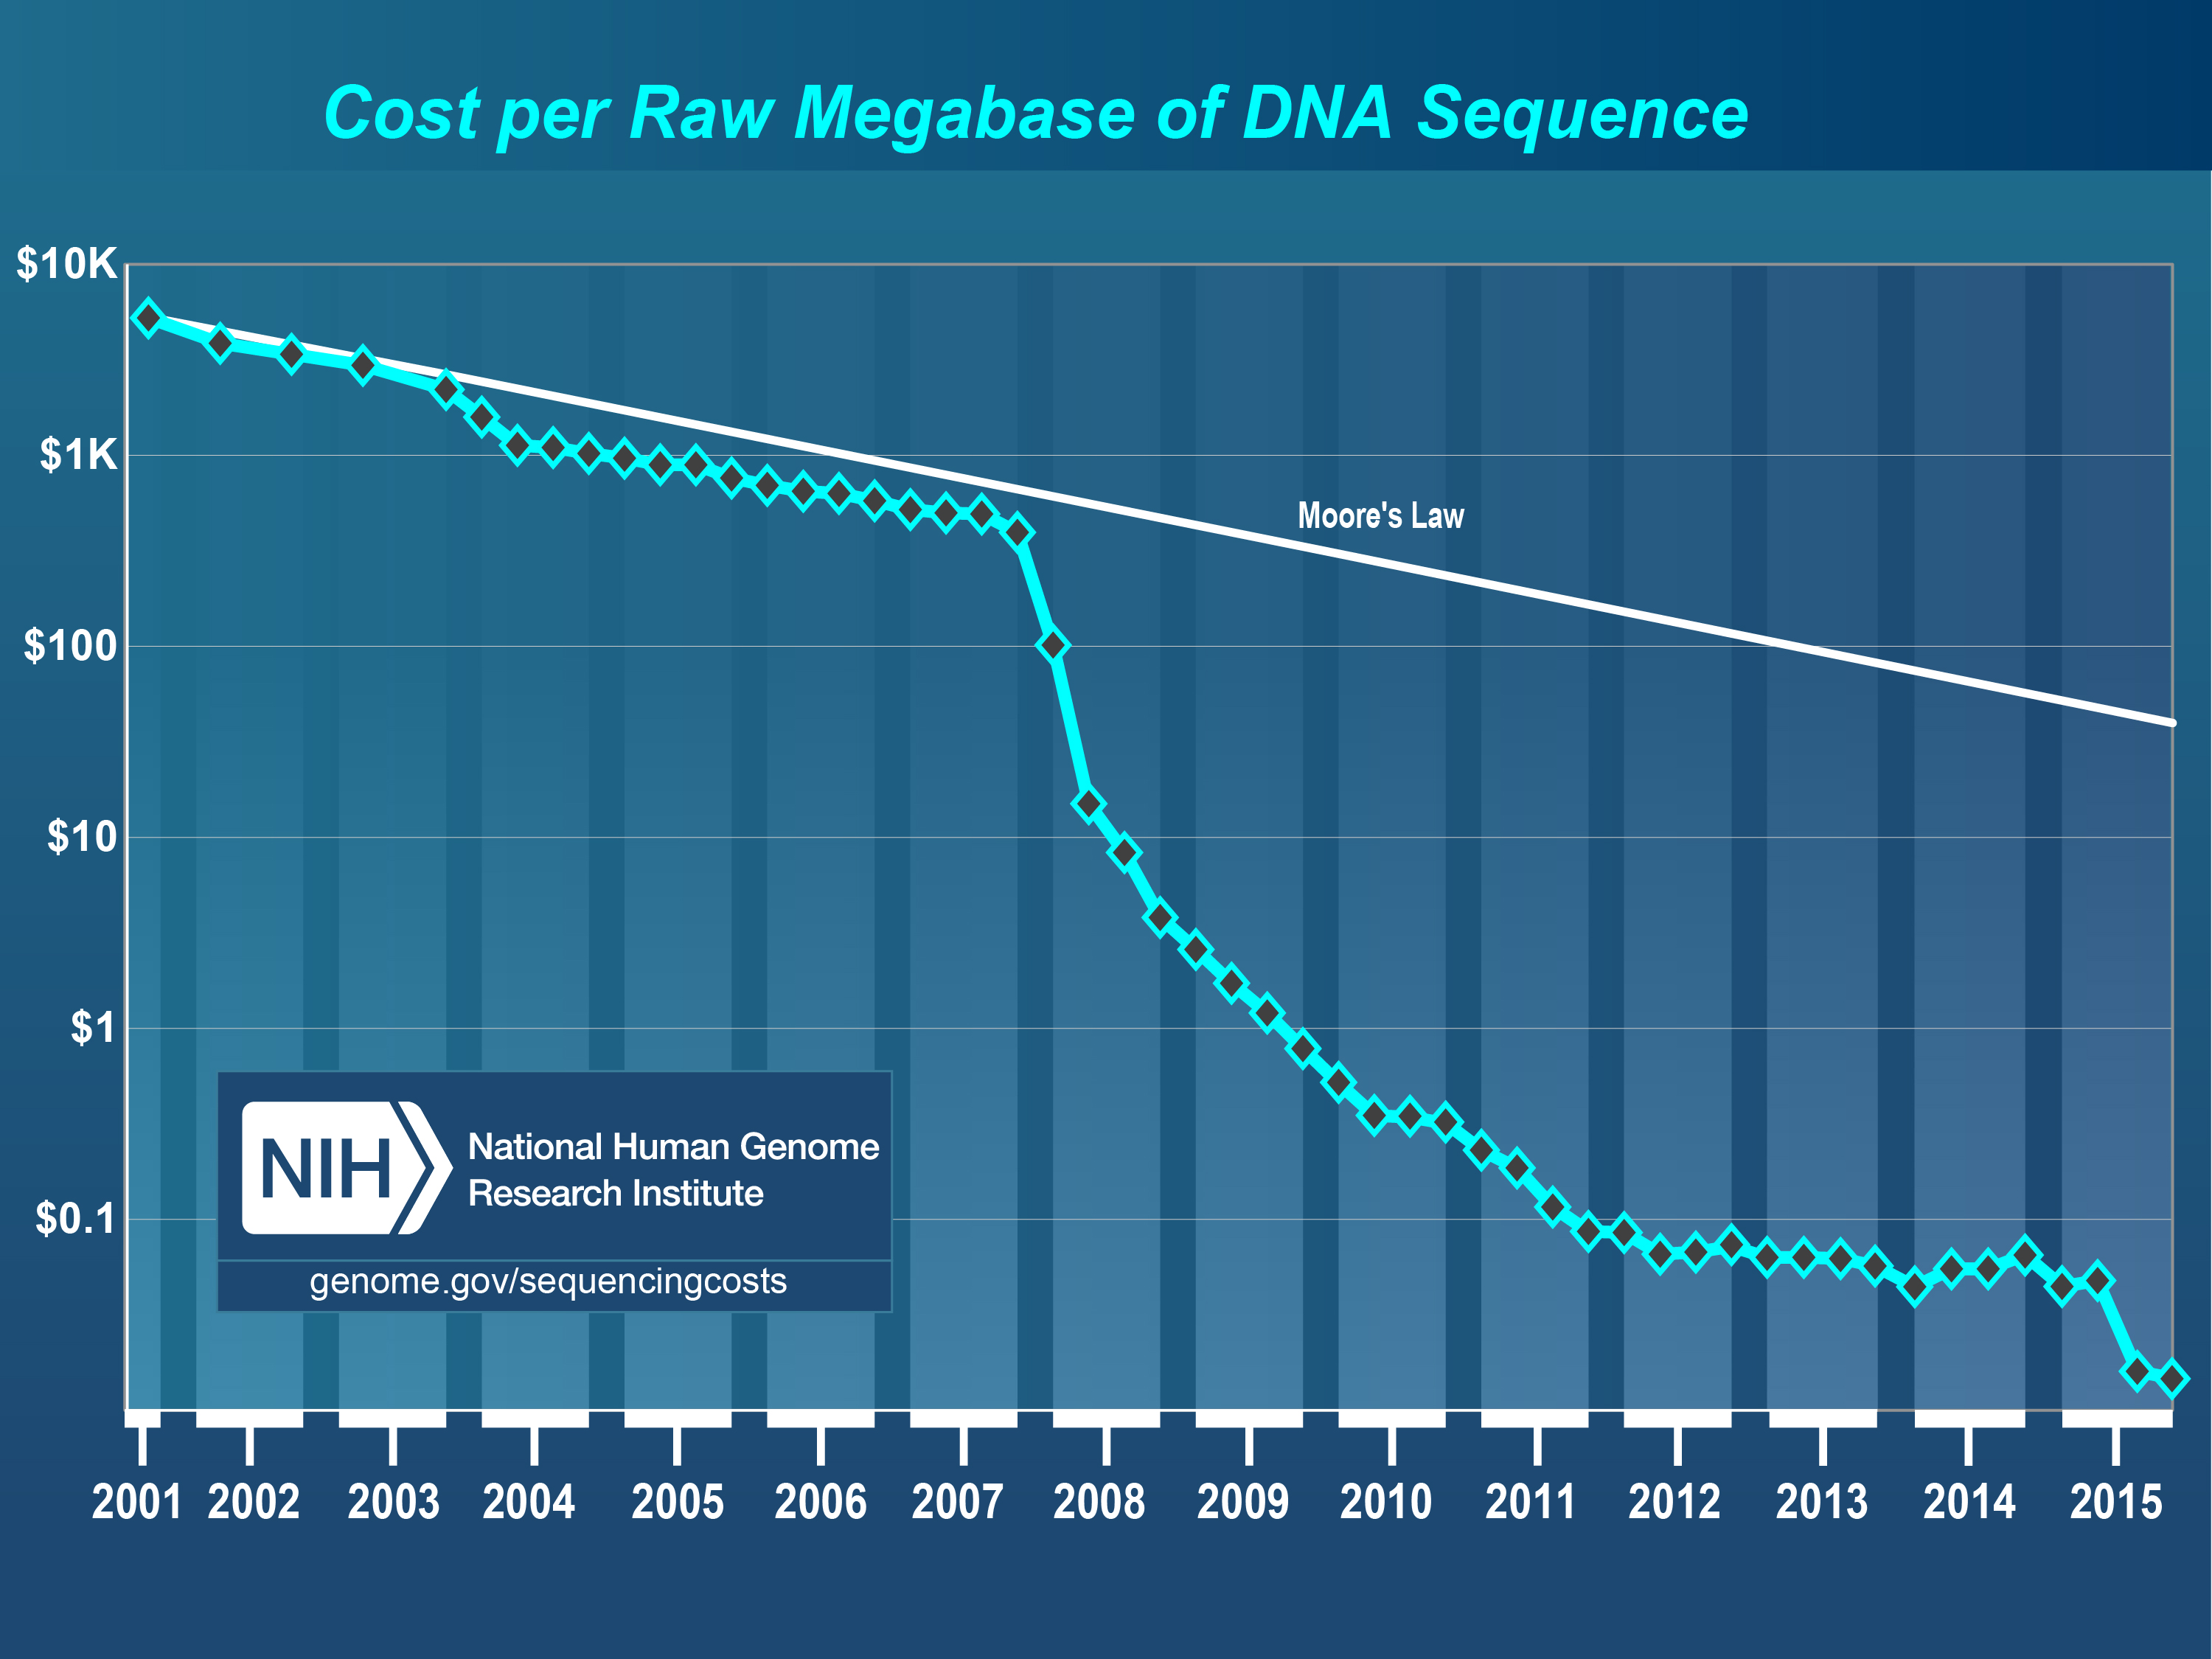
\includegraphics[width=0.8\linewidth]{images_20170829_NGS_cost.jpg}
\end{figure}
\end{frame}
%------------------------------------------------
\begin{frame}
\frametitle{Sequencing Output}
\begin{figure}
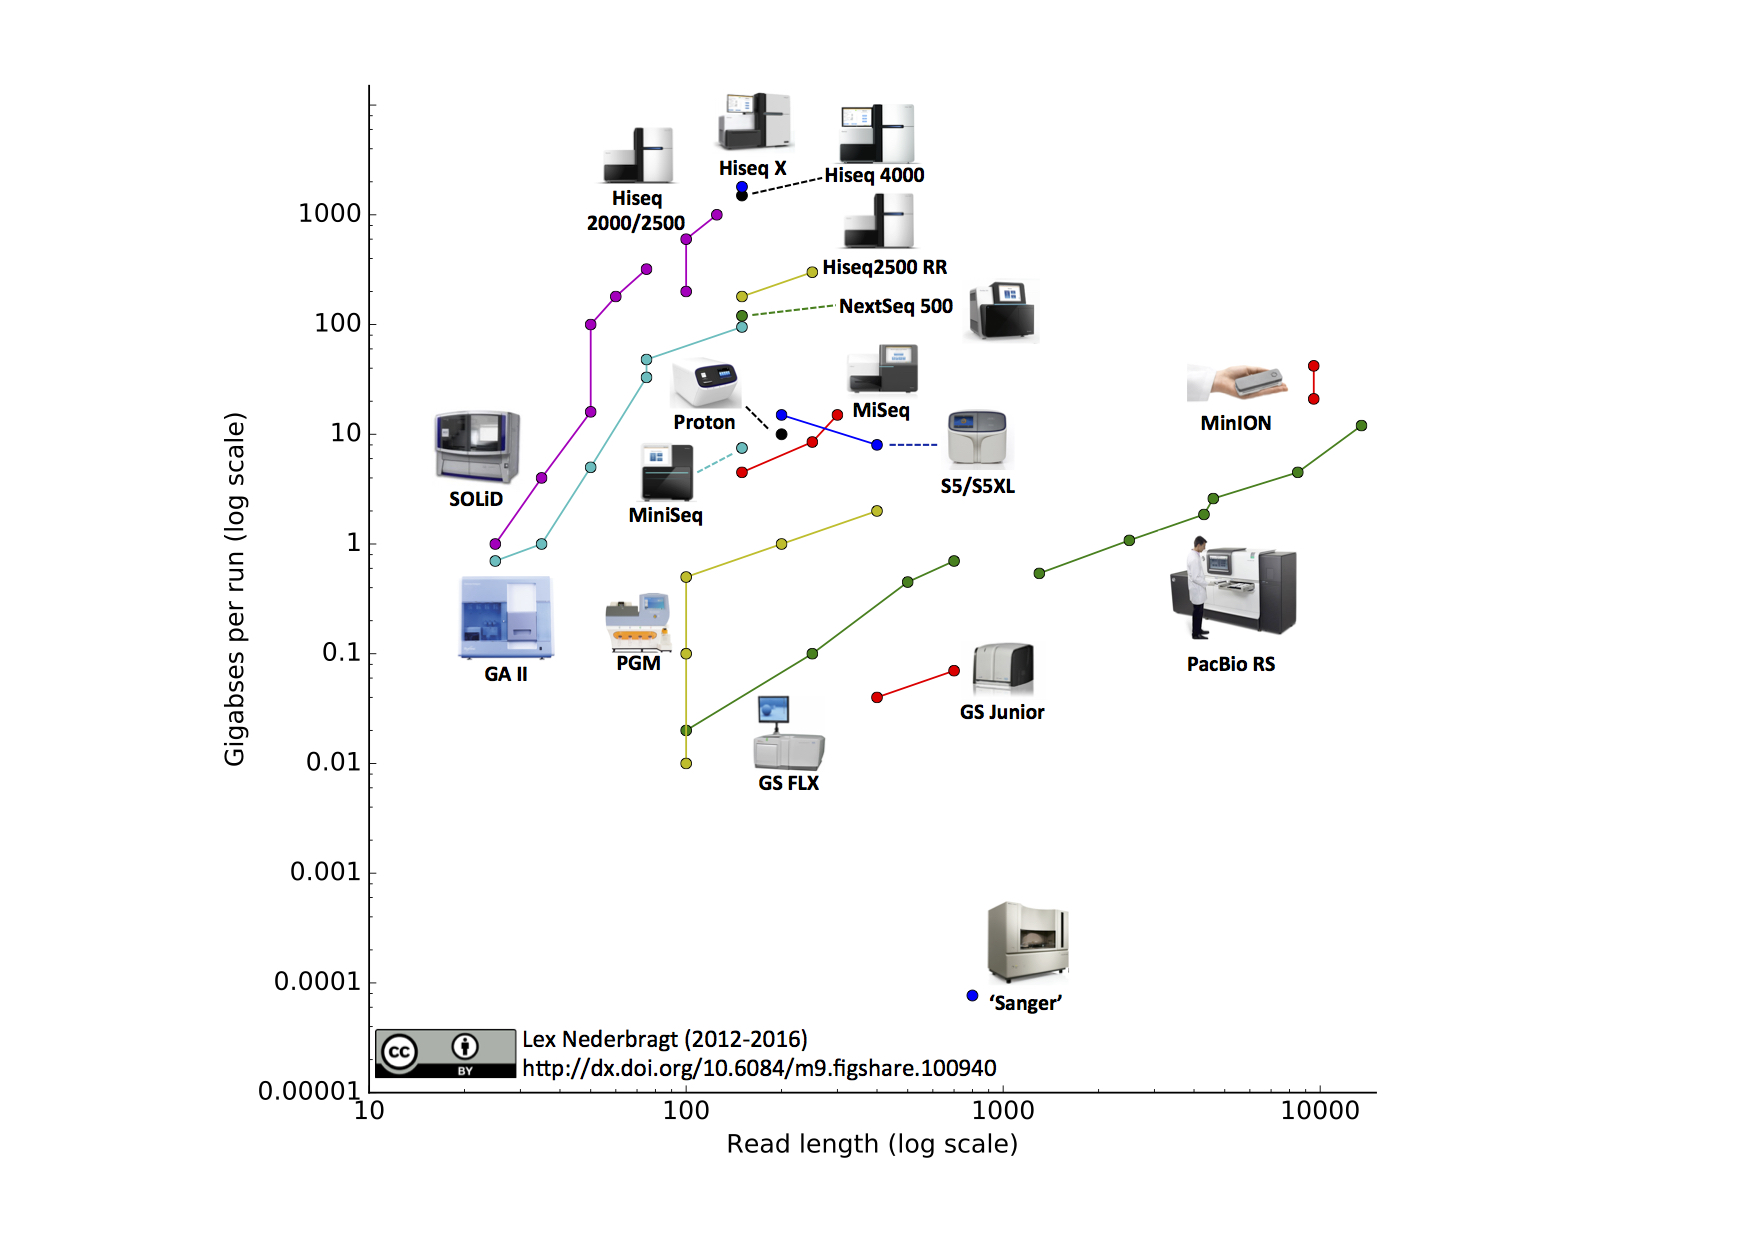
\includegraphics[width=0.8\linewidth]{images_20170829_machine_output.jpg}
\end{figure}
\end{frame}
%------------------------------------------------
\begin{frame}
\frametitle{Generational Shift}
\begin{itemize}
	\item<1-> More and more data can be generated cheaper
	\item<2-> Data length and quality are both improving
	\item<3-> How does this change the scope of research?
	\begin{itemize}
		\item<4-> (hint: Sanger is good for studying what?)
	\end{itemize}
\end{itemize}
\end{frame}
%------------------------------------------------
\begin{frame}
\frametitle{Course Motivations}
\begin{itemize}
	\item Biologist increasingly need to be programmers
	\item Topics often aren't introduced to undergraduates
	\item Cheap and Free Data
\end{itemize}
\end{frame}
%------------------------------------------------
\begin{frame}
\frametitle{Computational Need}
\begin{itemize}
	\item Biologist increasingly need to be programmers
	\item Many hypotheses are tested by generating piles of data
	\item Regardless of your future plans, programming and hypothesis testing are skills that all STEM students should have
\end{itemize}
%important for biologists to be programmers
\end{frame}
%------------------------------------------------
\begin{frame}
\frametitle{Cheap/Free Data}
\begin{figure}
\includegraphics <2-> [width=0.8\linewidth]{images_20170829_NGS_cost.jpg}
\end{figure}
\end{frame}
%------------------------------------------------
\begin{frame}
\frametitle{Cheap/Free Data}
\begin{itemize}
	\item Data is cheap and often free
	\item Computation is getting faster
	\item Combined, this means student projects are feasible
\end{itemize}
%how much? ncbi/sra chart
\end{frame}
%------------------------------------------------
\begin{frame}
\frametitle{Personal Experience}
\begin{itemize}
	\item Worked in Duke IGSP/CHGV Sequencing Core for 4 years
	\begin{itemize}
		\item Ran Illumina GA, GA2, HiSeq2000
	\end{itemize}
	\item PhD Thesis on Mouse Lemur Genomics
	\begin{itemize}
		\item Whole Genome Sequencing and Mutation Rate
		\item Rates of Sperm Gene Evolution
	\end{itemize}
\end{itemize}
%right in my wheelhouse
\end{frame}
%------------------------------------------------

\begin{frame}
\Huge{\centerline{The End}}
\end{frame}

%----------------------------------------------------------------------------------------

\end{document} 